\chapter{آزمایش و نتیجه}
در این فصل قصد داریم عملکرد و درستی روش ارائه‌شده در فصول ۴ و ۵ را با کمک آزمون‌های مختلف و شبیه‌سازی بررسی کنیم. در بخش نخست این فصل، به بررسی صحت مدل تعریف شده در مسئله خواهیم پرداخت. بدین منظور تاخیر سرویس بدست آمده توسط مدل تعریف شده را با نتیجه اجرای شبیه‌سازی بر روی همان مدل مقایسه خواهیم کرد. به عبارتی به کمک شبیه‌سازی مدل را با «خودش» مقایسه خواهیم کرد. در بخش دوم، به مقایسه عملکرد استراتژی بدست آمده توسط روش پیشنهادی با سایر استراتژی‌ها می‌پردازیم. در این بخش چندین استراتژی رایج را به عنوان استراتژی‌های پایه تعریف می‌کنیم و عملکرد استراتژی تخلیه پیشنهادی را در برابر آنها با کمک شبیه‌سازی بررسی می‌کنیم.
\section{بررسی صحت مدل}
در این بخش بررسی خواهیم کرد که آیا مقدار تاخیر سرویس بدست آمده توسط شبیه‌سازی با مقدار تاخیر مشخص شده در جواب بهینه مسئله‌ی 
$\mathcal{P}_2$
 (رابطه‌ی \ref{eq:p2}) همخوانی دارد یا نه. بدین منظور نتایج الگوریتم جستجوی استراتژی تخلیه را در دو سناریو شبیه‌سازی مختلف بررسی خواهیم کرد.
\subsection{سناریوی تک صف}
در این آزمون محیطی با یک صف وظیفه در نظر گرفته شده است که ویژگی‌های آن در جدول \ref{table:parameters-singlequeue} مشخص شده است. شبیه‌سازی به ازای ۲۹ مقدار مختلف $\eta_0$ صورت گرفته‌است که نتایج آن در مقایسه با مقدار محاسبه شده توسط مدل مسئله (برنامه خطی
$\mathcal{P}_2$
) در جدول \ref{table:scenario1} خلاصه شده است. تعداد سیکل‌های شبیه‌سازی در هر ۲۹ حالت برابر با $10^7$ بوده است. همانطور که مشاهده می‌شود مقدار تاخیر سرویس محاسبه شده توسط مدل برنامه‌ریزی خطی، بسیار نزدیک به مقدار تاخیر بدست آمده توسط شبیه‌سازی می‌باشد.
\begin{table}
	\centering
	\begin{latin}
		
		\begin{tabular}{rrrr}
			\hline
			\multicolumn{1}{l}{$\eta_1$} & \multicolumn{1}{l}{Delay (model estimate)} & \multicolumn{1}{l}{Delay (simulation result)} & \multicolumn{1}{l}{Error} \\ \hline
			0.01                     & 5.9403373                                  & 5.945382                                      & 0.0050447                 \\
			0.02                     & 5.9413582                                  & 5.9441002                                     & 0.002742                  \\
			0.03                     & 5.9873212                                  & 5.9979591                                     & 0.0106379                 \\
			0.04                     & 6.0332846                                  & 6.0445199                                     & 0.0112353                 \\
			0.05                     & 6.0792458                                  & 6.0772735                                     & -0.0019723                \\
			0.06                     & 6.1653313                                  & 6.1611952                                     & -0.0041361                \\
			0.07                     & 6.2608539                                  & 6.2771005                                     & 0.0162466                 \\
			0.08                     & 6.3563761                                  & 6.3485279                                     & -0.0078482                \\
			0.09                     & 6.4518981                                  & 6.4535551                                     & 0.001657                  \\
			0.1                      & 6.5474205                                  & 6.5470207                                     & -0.0003998                \\
			0.11                     & 6.6429429                                  & 6.6441015                                     & 0.0011586                 \\
			0.12                     & 6.7384654                                  & 6.7475386                                     & 0.0090732                 \\
			0.13                     & 6.8339881                                  & 6.8304343                                     & -0.0035538                \\
			0.14                     & 6.963416                                   & 6.967968                                      & 0.004552                  \\
			0.15                     & 7.117219                                   & 7.1221635                                     & 0.0049445                 \\
			0.16                     & 7.2710211                                  & 7.2660879                                     & -0.0049332                \\
			0.17                     & 7.4248235                                  & 7.4243839                                     & -0.0004396                \\
			0.18                     & 7.578626                                   & 7.5757626                                     & -0.0028634                \\
			0.19                     & 7.7324285                                  & 7.7334524                                     & 0.0010239                 \\
			0.2                      & 7.8862311                                  & 7.8823844                                     & -0.0038467                \\
			0.21                     & 8.0400334                                  & 8.0431362                                     & 0.0031028                 \\
			0.22                     & 8.193836                                   & 8.1896367                                     & -0.0041993                \\
			0.23                     & 8.3476384                                  & 8.3507161                                     & 0.0030777                 \\
			0.24                     & 8.5014409                                  & 8.50166                                       & 0.0002191                 \\
			0.25                     & 8.6793609                                  & 8.6778177                                     & -0.0015432                \\
			0.26                     & 8.9366602                                  & 8.9342996                                     & -0.0023606                \\
			0.27                     & 9.334054                                   & 9.3359713                                     & 0.0019173                 \\
			0.28                     & 9.9963099                                  & 9.9920628                                     & -0.0042471                \\
			0.29                     & 11.6247515                                 & 11.6247351                                    & -0.0000164                \\ \hline
			\multicolumn{3}{r}{Variance}                                                                                          & 0.0000314                 \\
			\multicolumn{3}{r}{Mean absolute difference}                                                                          & 0.0041032                 \\ \hline
		\end{tabular}
	\end{latin}
	\caption{مقایسه‌ی میزان تاخیر بدست آمده از مدل و شبیه‌سازی در سناریوی تک صف}
	\label{table:scenario1}
\end{table}

\subsection{سناریوی دو صف}
در این آزمون محیطی با دو صف وظیفه در نظر گرفته شده است که ویژگی‌های آن در جدول \ref{table:fixedranged} مشخص شده است. شبیه‌سازی به ازای ۲۲ مقداردهی مختلف به $\eta_1, \eta_2$ صورت گرفته‌است که نتایج آن در مقایسه با مقدار محاسبه شده توسط مدل مسئله در جدول \ref{table:scenario2} خلاصه شده است. تعداد سیکل‌های شبیه‌سازی در هر ۲۹ حالت برابر با $10^7$ بوده است. همانطور که مشاهده می‌شود مقدار تاخیر سرویس محاسبه شده توسط مدل برنامه‌ریزی خطی، بسیار نزدیک به مقدار بدست آمده توسط شبیه‌سازی می‌باشد.
% Please add the following required packages to your document preamble:
% \usepackage{booktabs}
\begin{table}[]
	\centering
	\begin{latin}
		\begin{tabular}{@{}rrrrr@{}}
			\toprule
			\multicolumn{1}{l}{$\eta_1$} & \multicolumn{1}{l}{$\eta_2$} & \multicolumn{1}{l}{Delay (model estimate)} & \multicolumn{1}{l}{Delay (simulation result)} & \multicolumn{1}{l}{Error} \\ \midrule
			0                        & 0                        & 5.3055545                                  & 5.3043168                                     & -0.0012377                \\
			0                        & 0.2                      & 4.5749717                                  & 4.5740879                                     & -0.0008838                \\
			0                        & 0.4                      & 4.2116748                                  & 4.2124139                                     & 0.0007391                 \\
			0                        & 0.6                      & 3.9532195                                  & 3.954735                                      & 0.0015155                 \\
			0                        & 0.8                      & 3.6947642                                  & 3.6941737                                     & -0.0005905                \\
			0                        & 1                        & 3.4702381                                  & 3.4711606                                     & 0.0009225                 \\
			0.2                      & 0                        & 5.4240034                                  & 5.425082                                      & 0.0010786                 \\
			0.2                      & 0.2                      & 4.9543158                                  & 4.9546973                                     & 0.0003815                 \\
			0.2                      & 0.4                      & 4.7082897                                  & 4.7077916                                     & -0.0004981                \\
			0.2                      & 0.6                      & 4.5023325                                  & 4.5033802                                     & 0.0010477                 \\
			0.2                      & 0.8                      & 4.3225922                                  & 4.3218913                                     & -0.0007009                \\
			0.2                      & 1                        & 4.3916784                                  & 4.3898362                                     & -0.0018422                \\
			0.4                      & 0                        & 6.0300612                                  & 6.0294958                                     & -0.0005654                \\
			0.4                      & 0.2                      & 5.6038029                                  & 5.6044667                                     & 0.0006638                 \\
			0.4                      & 0.4                      & 5.3794469                                  & 5.3817302                                     & 0.0022833                 \\
			0.4                      & 0.6                      & 5.1951134                                  & 5.1951965                                     & 0.0000831                 \\
			0.4                      & 0.8                      & 5.1865812                                  & 5.1870742                                     & 0.000493                  \\
			0.4                      & 1                        & 5.4041958                                  & 5.4026623                                     & -0.0015335                \\
			0.6                      & 0                        & 7.4340974                                  & 7.4330417                                     & -0.0010557                \\
			0.6                      & 0.2                      & 7.2298104                                  & 7.2298944                                     & 0.000084                  \\
			0.6                      & 0.4                      & 7.5736237                                  & 7.5743988                                     & 0.0007751                 \\
			0.6                      & 0.6                      & 8.7051662                                  & 8.7024916                                     & -0.0026746                \\ \midrule
			\multicolumn{4}{r}{Variance}                                                                                                                     & 0.0000314                 \\
			\multicolumn{4}{r}{Mean absolute difference}                                                                                                     & 0.0041032                 \\ \bottomrule
		\end{tabular}
	\end{latin}
	\caption{مقایسه‌ی میزان تاخیر بدست آمده از مدل و شبیه‌سازی در سناریوی دو صف}
	\label{table:scenario2}
\end{table}
\section{بررسی عملکرد در مقایسه با استراتژی‌های پایه}
در این بخش عملکرد استراتژی یافت شده توسط الگوریتم \ref{alg:cap} را با چهار الگوریتم پایه زیر مقایسه می‌کنیم:
\begin{enumerate}
	\item استراتژی «فقط تخلیه»\LTRfootnote{Offload Only} که همه‌ی وظایف را تخلیه می‌کند
	\item استراتژی «حریصانه، تخلیه اول»\LTRfootnote{Greedy (Offload First)} که در هر بازه زمانی اگر واحد ارسال یا پردازنده بیکار باشند به هر کدام از آنها یک وظیفه از صفی رندوم تخصیص می‌دهد و در صورتی که تنها یک وظیفه در صف باشد و مجبور به انتخاب بین تخلیه و اجرای محلی باشد، تخلیه را انتخاب می‌کند.
	\item استراتژی «حریصانه، محلی اول»\LTRfootnote{Greedy (Local First)} که در هر بازه زمانی اگر واحد ارسال یا پردازنده بیکار باشند به هر کدام از آنها یک وظیفه از صفی رندوم تخصیص می‌دهد و در صورتی که تنها یک وظیفه در صف باشد و مجبور به انتخاب بین تخلیه و اجرای محلی باشد، اجرای محلی را انتخاب می‌کند.
	\item استراتژی «فقط (اجرای) محلی»\LTRfootnote{Local Only}
\end{enumerate}
\subsection{شبیه‌سازی تک صف}
با توجه به اینکه روش ارائه‌شده توسط ما حالت گسترش یافته \cite{Liu} است، ابتدا محیط آزمایش ارائه‌شده در آن پژوهش را برای آزمون الگوریتم در نظر می‌گیریم. پارامترهای این محیط در جدول \ref{table:parameters-singlequeue} خلاصه شده اند. نتیجه این آزمایش در شکل \ref{plot:singleQueue} مشاهده می‌شود.

% Please add the following required packages to your document preamble:
\begin{table}
	\centering
	\begin{latin}
		\begin{tabular}{@{}lllllllll@{}}
			\toprule
			\textbf{Parameter} & $M_1$ & $L_1$ & $\beta$ & $P_{tx}$ & $P_{loc}$ & $P_{max}$ & $C_1$ & $t_{rx}$ \\ \midrule
			\textbf{Value}             & 1    & 17   & 0.4  & 1.0 & 0.8  & 1.6  & 1    & 0.0   \\ \bottomrule
		\end{tabular}
	\end{latin}
	\caption{پارامترهای محیط رایانش لبه‌ای در سناریوی تک صف}
	\label{table:parameters-singlequeue}
\end{table}

\begin{figure}
	\centering
	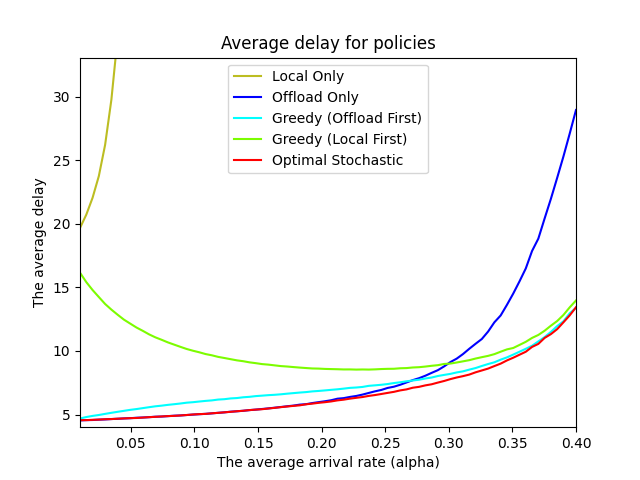
\includegraphics[width=0.7\textwidth]{PlotLiuLimitedSingleQueue.png}
	\caption{تاخیر سرویس بر حسب نرخ ورود در حالت تک صف}{تاخیر سرویس بر حسب نرخ ورود $\alpha_1$ در حالت تک صف}
	\label{plot:singleQueue}
\end{figure}
همانطور که مشاهده می‌شود استراتژی تخلیه تصادفی یافت شده از تمام الگوریتم‌های پایه بهتر عمل می‌کند و شکل منحنی‌های نمودار با \cite{Liu} مطابقت دارد.
\subsection{شبیه‌سازی دو صف با یک صف ثابت در سناریوی سبک و سنگین}
در این قسمت سناریوی آزمون به این گونه است که میزان تاخیر به ازای مقادیر مختلف نرخ ورود برای صف شماره یک و مقدار ثابت نرخ ورود برای صف شماره دو مشاهده می‌شود. پارامترهای محیطی در نظر گرفته شده در جدول \ref{table:fixedranged} به طور خلاصه آمده است.
\begin{figure}
	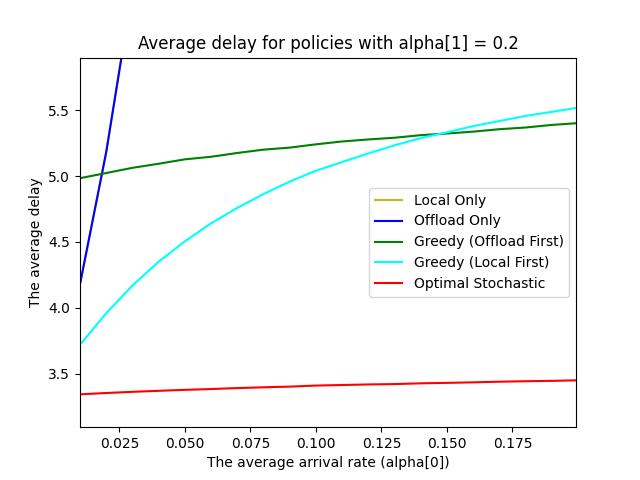
\includegraphics[width=\textwidth]{FixedRanged.png}
\end{figure}
% Please add the following required packages to your document preamble:
% \usepackage{booktabs}
\begin{table}
	\centering
	\begin{latin}
		\begin{tabular}{@{}llllllllllll@{}}
			\toprule
			\textbf{Parameter} & $M_1$ & $M_2$ & $L_1$ & $L_2$ & $C_1$ & $C_2$ & $\beta$ & $P_{tx}$ & $P_{loc}$ & $P_{max}$ & $t_{rx}$ \\ \midrule
			\textbf{Value}     & 1     & 3     & 7     & 2     & 1     & 1     & 0.95    & 1        & 0.8       & 1.6       & 0        \\ \bottomrule
		\end{tabular}
	\end{latin}
	\caption{پارامترهای محیط رایانش لبه‌ای در سناریوی دو صف با یک صف ثابت}
	\label{table:fixedranged}
\end{table}
همانطور که مشاهده می‌شود استراتژی تخلیه‌ی بهینه بسیار بهتر از الگوریتم‌های پایه عمل می‌کند. دلیل اصلی این تفاوت زیاد (نسبت به تفاوت کم در سناریوی با یک صف در بخش قبل) عدم هوشمندی استراتژی‌های حریصانه در انتخاب نوع وظیفه‌ی تخصیص داده شده به پردازنده و واحد ارسال است. به عبارت دیگر انتخاب تصادفی نوع وظیفه فرستاده شده به پردازنده و واحد ارسال در الگوریتم‌های حریصانه باعث می‌شود که در شرایطی که تفاوت زیادی بین نوع وظایف وجود دارد (مانند سناریو سبک و سنگین) این الگوریتم‌ها عملکرد خیلی بدی داشته باشند. این در حالی است که در حالت تک صف انتخاب بین انواع وظیفه مطرح نبوده است و تنها عامل برای عملکرد غیربهینه‌ی استراتژی‌های حریصانه، عدم زمانبندی درست وظایف بوده است.
\subsection{شبیه‌سازی دو صف متغیر وظایف سبک و سنگین}
\label{sub:heavylight}
در این قسمت مقدار تاخیر سرویس به ازای مقادیر مختلف نرخ ورود به هر دو صف محاسبه شده است. پارامترهای سیستمی این سناریو در جدول \ref{table:double} آمده است. همانطور که مشاهده می‌شود استراتژی بهینه در بازه 
$\alpha_1, \alpha_2 \in [0, 0.4]$
عملکرد قابل قبول دارد.
\begin{figure}[H]
	\centering
	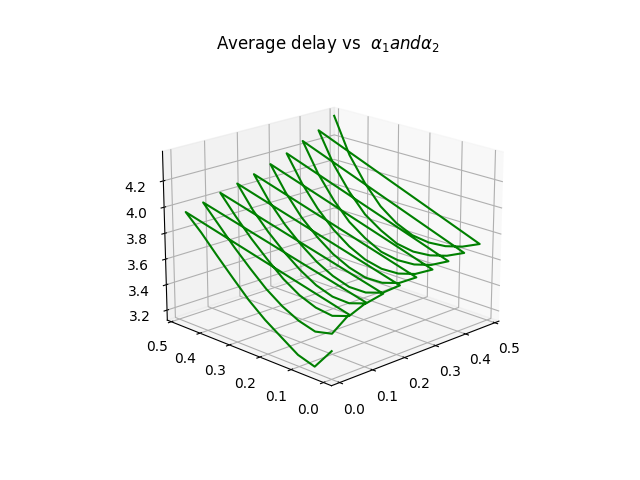
\includegraphics[width=0.7\textwidth]{Plot3d.png}
	\caption[تاخیر سرویس بر حسب نرخ ورود در حالت دو صف]{تاخیر سرویس بر حسب نرخ ورود $\alpha_1$ و $\alpha_2$ در حالت دو صف}
\end{figure}
\newpage
\begin{table}[H]
	\centering
	\begin{latin}
		\begin{tabular}{@{}llllllllllll@{}}
			\toprule
			\textbf{Parameter} & $M_1$ & $M_2$ & $L_1$ & $L_2$ & $C_1$ & $C_2$ & $\beta$ & $P_{tx}$ & $P_{loc}$ & $P_{max}$ & $t_{rx}$ \\ \midrule
			\textbf{Value}     & 1     & 3     & 7     & 2     & 1     & 1     & 0.95    & 1        & 0.8       & 1.6       & 0        \\ \bottomrule
		\end{tabular}
	\end{latin}
	\caption{پارامترهای محیط رایانش لبه‌ای در سناریوی دو صف متغیر}
	\label{table:double}
\end{table}
\subsection{شبیه‌سازی سه صف وظیفه}
\label{sec:effectiveness}
در این قسمت عملکرد الگوریتم ارائه‌شده در شرایطی که سه صف وجود دارد بررسی شده است. پارامترهای محیط رایانش لبه‌ای در جدول \ref{table:triple} آورده شده است. با توجه به اینکه رسم نمودار در شرایط چهار بعدی امکان‌پذیر نیست از مفهومی به نام آزمون «کارآمدی» استفاده می‌کنیم. مفهوم کارآمدی را اینگونه تعریف می‌کنیم که یک استراتژی کارآمد است اگر احتمال پر بودن یک یا چند صف در سیستم از 
$\frac{1}{|S|}$
کمتر باشد. در این آزمایش، کارآمدی استراتژی‌های مختلف را به ازای ۱۰۰۰ نمونه مختلف در بازه‌های 
$\alpha_1, \alpha_2, \alpha_3 \in [0, 0.2]$
 آزمایش کردیم که نتایج آن در جدول \ref{table:triplequeuepercents} مشاهده می‌شود.
 
\begin{table}[H]
	\centering
	\begin{latin}		
		\resizebox{\textwidth}{!}{
		\begin{tabular}{llllll}
			\hline
			\textbf{Policy} & Optimal & Local Only & Greedy (Local First) & Greedy (Offload First) & Offload Only \\ \hline
			\textbf{Effectiveness}           & 100.0\%   & 8.5\%      & 80.3\%                & 79.3\%                  & 21.6\%        \\ \hline
		\end{tabular}
	}
	\end{latin}
	\caption{ درصد کارآمدی استراتژی‌ها}
	\label{table:triplequeuepercents}
\end{table}

% Please add the following required packages to your document preamble:
% \usepackage{booktabs}
\begin{table}[H]
	\centering
	\resizebox{\textwidth}{!}{
	\begin{latin}		
		\begin{tabular}{@{}lllllllllllllll@{}}
			\toprule
			Parameter & $M_1$ & $M_2$ & $M_3$ & $L_1$ & $L_2$ & $L_3$ & $C_1$ & $C_2$ & $C_3$ & $\beta$ & $P_{tx}$ & $P_{loc}$ & $P_{max}$ & $t_{rx}$ \\ \midrule
			Value     & 1     & 3     & 2     & 4     & 2     & 3     & 1     & 1     & 2     & 0.95    & 1        & 0.8       & 1.6       & 0.5      \\ \bottomrule
		\end{tabular}
	\end{latin}
		}
	\caption{پارامترهای محیط رایانش لبه‌ای در سناریوی سه صف}
	\label{table:triple}
\end{table}
\newpage
\section{آزمون کارآیی}
یک نکته که در دو بخش پیشین به آن اشاره‌ای نشد کارایی الگوریتم ارائه‌شده از نظر زمان اجرا و حافظه مصرفی می‌باشد. در آزمایش‌های بخش پیشین تعداد صف‌ها ۳ یا کمتر در نظر گرفته شده بود که اجرای الگوریتم مسئله را به راحتی میسر می‌ساخت. دلیل این امر این است که با افزایش تعداد صف‌ها، فضای حالت مسئله به صورت نمایی بزرگ خواهد شد. در جدول \ref{table:statespace} تعداد حالت‌های زنجیره‌ی مارکوف $|S|$ به همراه زمان اجرا و حافظه مصرفی لازم جهت حل مسئله آورده شده است. برای تفسیر راحت‌تر نتایج آزمایش، تعداد بسته‌ها و قسمت‌های تمام صف‌ها برابر مقدار ثابت $L_i = M_i = 2$ در نظر گرفته شده است. البته در شرایط واقعی قطعا تعداد قسمت‌ها و بسته‌‌های هر صف متفاوت خواهند بود. زیرا در غیر این صورت صف‌های با ویژگی‌های یکسان را می‌توان به یک صف با نرخ ورود مجموع تبدیل کرد. پردازنده استفاده شده در این آزمایش \lr{Intel® Xeon® Processor E3-1220} بوده است. حل‌کننده خطی استفاده شده \lr{GLOP} بوده است\footnote{در آزمایش‌های انجام شده مشاهده شد که \lr{GLOP} عملکرد بهتری نسبت به \lr{CPLEX} دارد و به این دلیل انتخاب گردید}. طول هر وظیفه برابر با $Q = 6$ در نظر گرفته شده است. همانطور که مشاهده می‌شود زمان اجرای الگوریتم به صورت نمایی افزایش می‌یابد و مسئله فقط برای تعداد صف‌های کمتر از ۵ در زمان قابل قبول حل می‌شود. این تعداد در محیط‌های با تنوع وظایف نسبتا کم مانند سناریوی «سبک»‌ «سنگین» که پیشتر بیان شد، انتزاع قابل قبولی از فضای مسئله ارائه می‌دهد و عملکرد بهتری از حالت تک وظیفه دارد. در فصل پیش رو چندین ایده که می‌تواند در کاهش فضای حالت مسئله و بهبود عملکرد الگوریتم موثر باشد، جهت پژوهش بیشتر ارائه‌شده اند.
% Please add the following required packages to your document preamble:
% \usepackage{booktabs}
\begin{table}[H]
	\centering
	\begin{latin}
\begin{tabular}{@{}lll@{}}
	\toprule
	Number of queues & State count ($|S|$) & Running time                  \\ \midrule
	1                & 14                & 80ms                          \\
	2                & 147               & 433ms                         \\
	3                & 1372              & 7003 ms                       \\
	4                & 100842            & 24164 seconds ($\sim$7 Hours) \\ \bottomrule
\end{tabular}
	\end{latin}
	\caption{زمان اجرا و اندازه‌ی فضای حالت به ازای تعداد صف $k = 1, 2, 3, 4$}
	\label{table:statespace}
\end{table}
\clearpage
